\chapter[Implementação do sistema de supervisório]{Implementação do Sistema de supervisório}

Neste capítulo serão apresentados a implementação do projeto e os resultados obtidos com o interfaceamento do supervisório.


\section{Interfaceamento do protótipo com o supervisório}

Ao realizar o login no sistema, o primeiro item a ser tratado é a adição de novos datasources.

Para adicionar um datasource no tipo Modbus RTU no SCADABR, o primeiro passo é acessar a interface do sistema e fazer o login. Uma vez logado, vá até o menu superior e selecione a opção Datasources para gerenciar as fontes de dados disponíveis. Na nova tela, escolha a opção Adicionar Fonte de Dados e, entre as alternativas apresentadas, selecione Modbus Serial, que corresponde ao protocolo RTU.

Após selecionar o tipo Modbus Serial, você será direcionado para a tela de configuração do novo datasource. Nesta etapa, será necessário preencher algumas informações importantes para garantir que a comunicação com o dispositivo Modbus RTU funcione corretamente. A primeira parte é atribuir um nome ao datasource, de forma que ele seja facilmente identificado, como por exemplo "Controlador de Motor Modbus RTU". Em seguida, defina a porta serial à qual o dispositivo está conectado, como /dev/ttyUSB0 no caso de sistemas Linux, ou COM3 se estiver utilizando Windows.

A configuração da taxa de comunicação, ou baud rate, é crucial e deve corresponder à configuração do dispositivo escravo. O valor selecionado é de 9600 bps, . O número de bits é 8N\&1 e o bit de paridade é 0, o timeou por padrão é de 500ms, mas para a melhor leitura, será colocado 1000ms.

Logo após, serão lidos cada ponto de leitura, de acordo com o registrador adicionado. A leitura é fundamental para saber se os registradores estão respondendo. Por último, cada datasource será colocado e adicionado para a observação no \textit{watchlist}.

Após acessar e testar as variáveis do \textit{watchlist} é preciso criar um novo Dashboard ou Tela de Visualização.

Na tela de criação do dashboard, você terá a opção de definir um nome para sua nova tela, algo que ajude a identificar seu propósito, como "Controle de Temperatura" ou "Monitoramento de Motores". Após definir o nome, você pode começar a adicionar elementos à tela, como gráficos, indicadores, botões e outros componentes que ajudarão na visualização dos dados.

Para adicionar um componente, clique em Adicionar Componente ou arraste e solte o item desejado da biblioteca de widgets para a área de edição do dashboard. Os componentes incluem gráficos, medidores, tabelas e outros elementos visuais que podem ser configurados para exibir dados provenientes dos datasources que você configurou anteriormente.

Depois de adicionar um componente, é necessário configurá-lo. Para isso, será ncecessário clilcar sobre o componente para abrir as opções de configuração. Defina as propriedades necessárias, como a fonte dos dados, o tipo de gráfico ou indicador, e quaisquer outras configurações específicas. Por exemplo, para um gráfico, você precisará selecionar o datasource e configurar os parâmetros de visualização, como os eixos e a escala.

Com os componentes configurados, ajuste o layout e o tamanho dos itens na tela para que eles fiquem organizados e visualmente agradáveis. Finalmente, após configurar todos os componentes e ajustar o layout, será necessário salvar as alterações no dashboard. 

\begin{figure}[h]
	\centering
	\label{fig:Pocos_scada}
		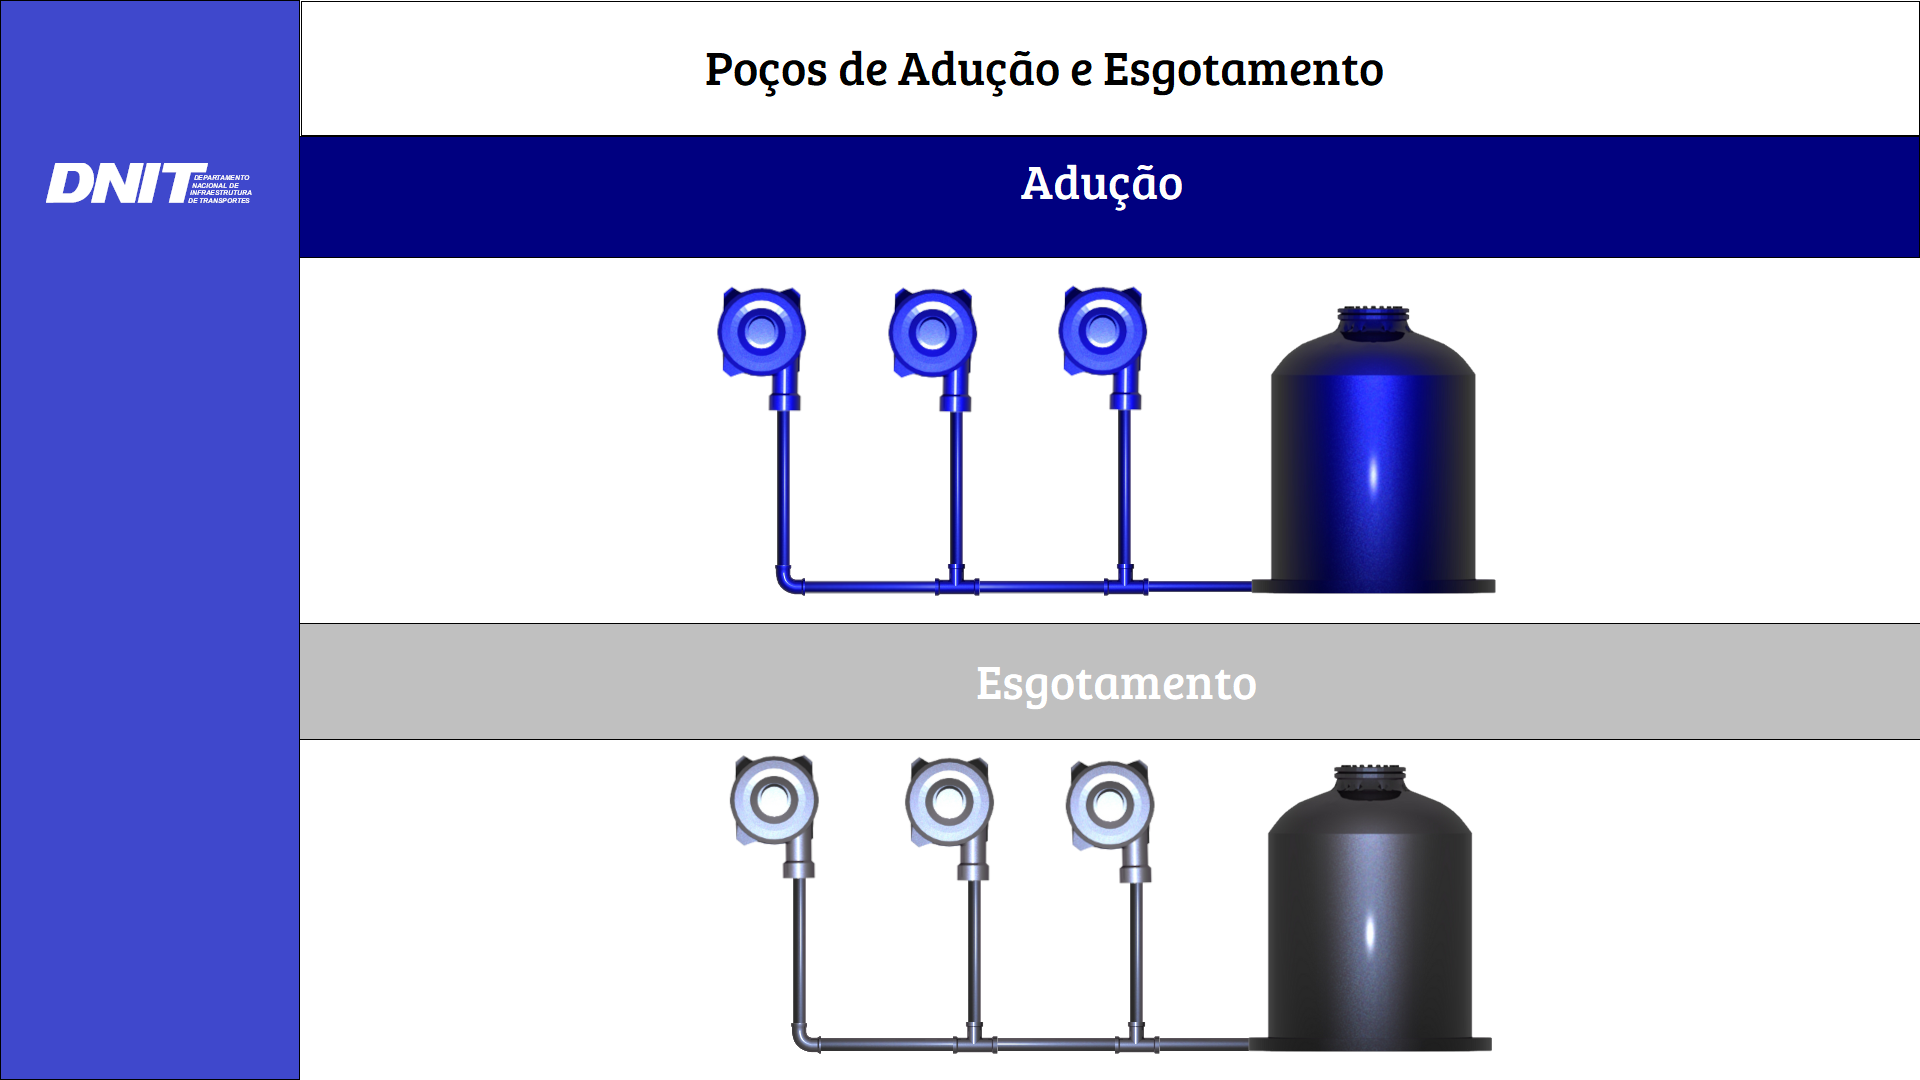
\includegraphics[keepaspectratio=true,scale=0.2]{figuras/Supervisorio.png}
	\caption{Dashboard dos motores dos poços}
\end{figure}

\begin{figure}[h]
	\centering
	\label{fig:sem_scada}
		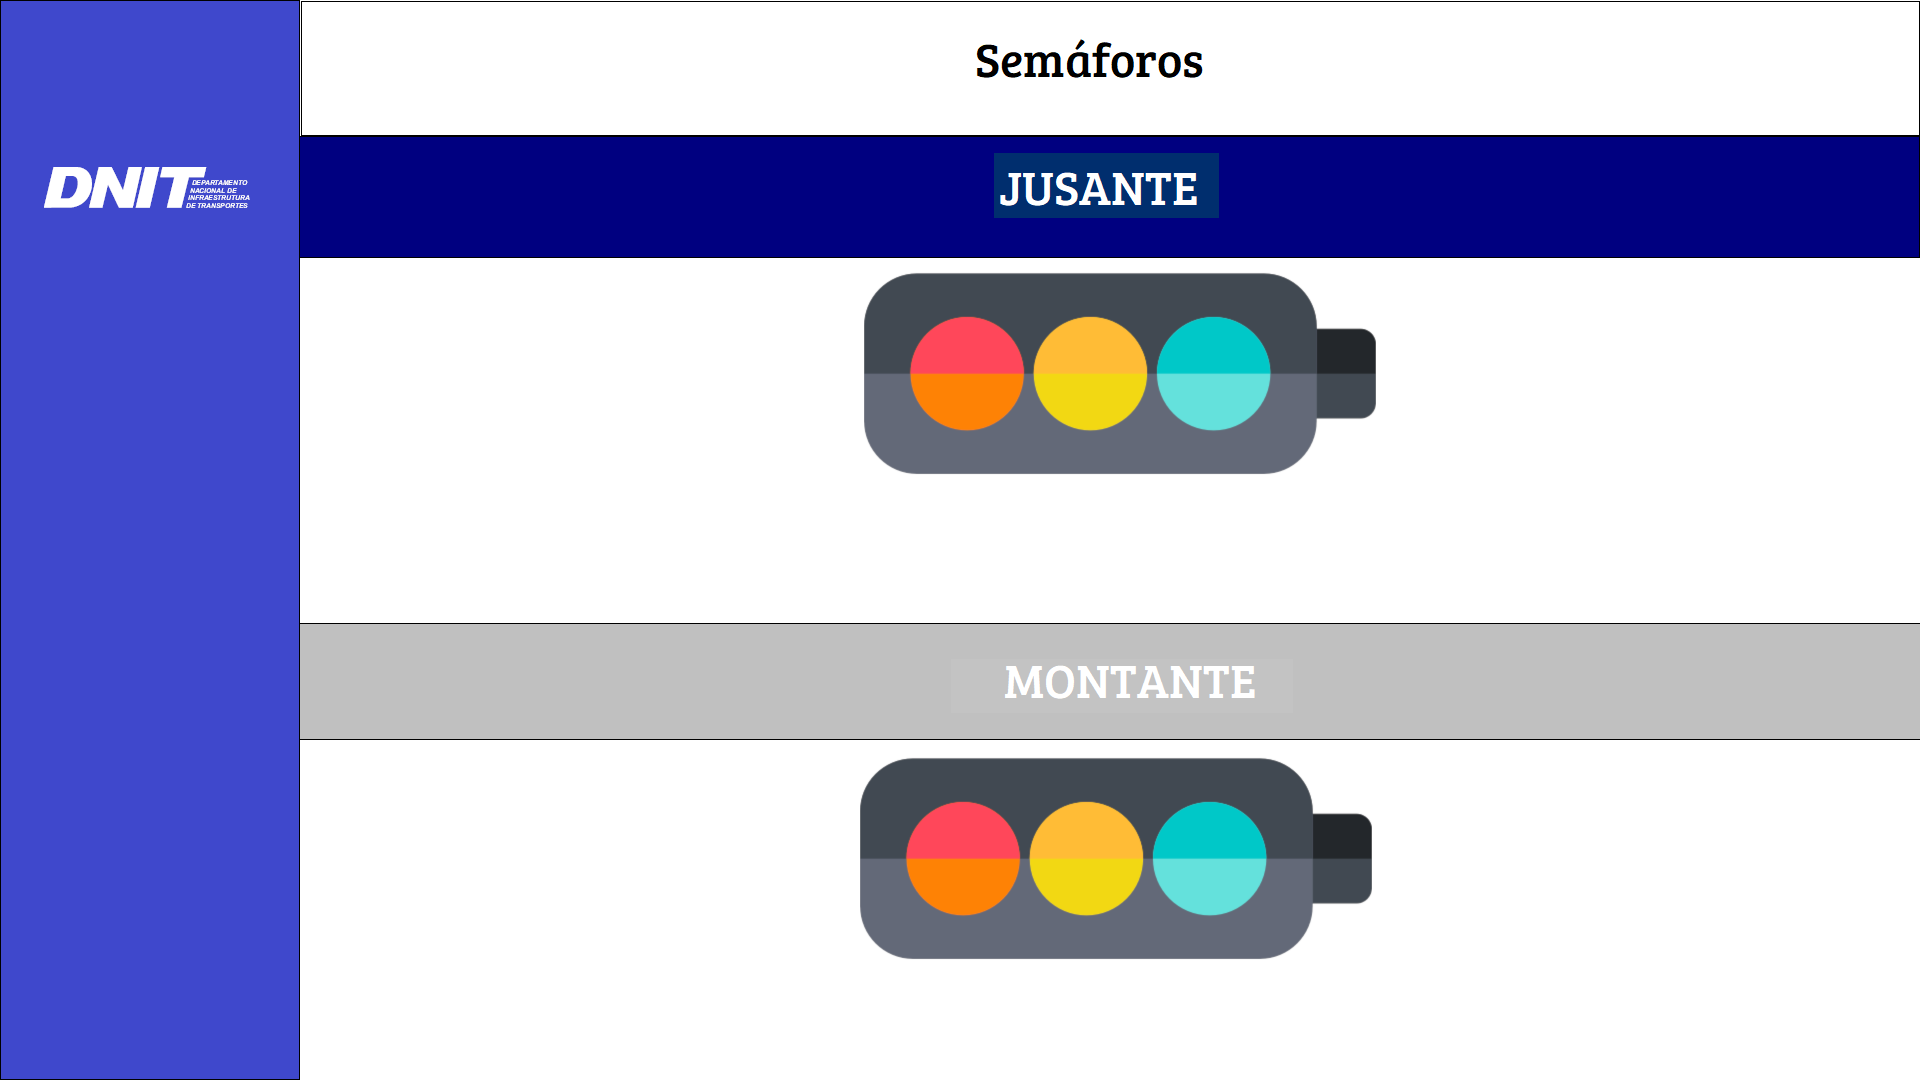
\includegraphics[keepaspectratio=true,scale=0.2]{figuras/Semáforos.png}
	\caption{Dashboard dos semáforos}
\end{figure}

\begin{figure}[h]
	\centering
	\label{fig:ponte_scada}
		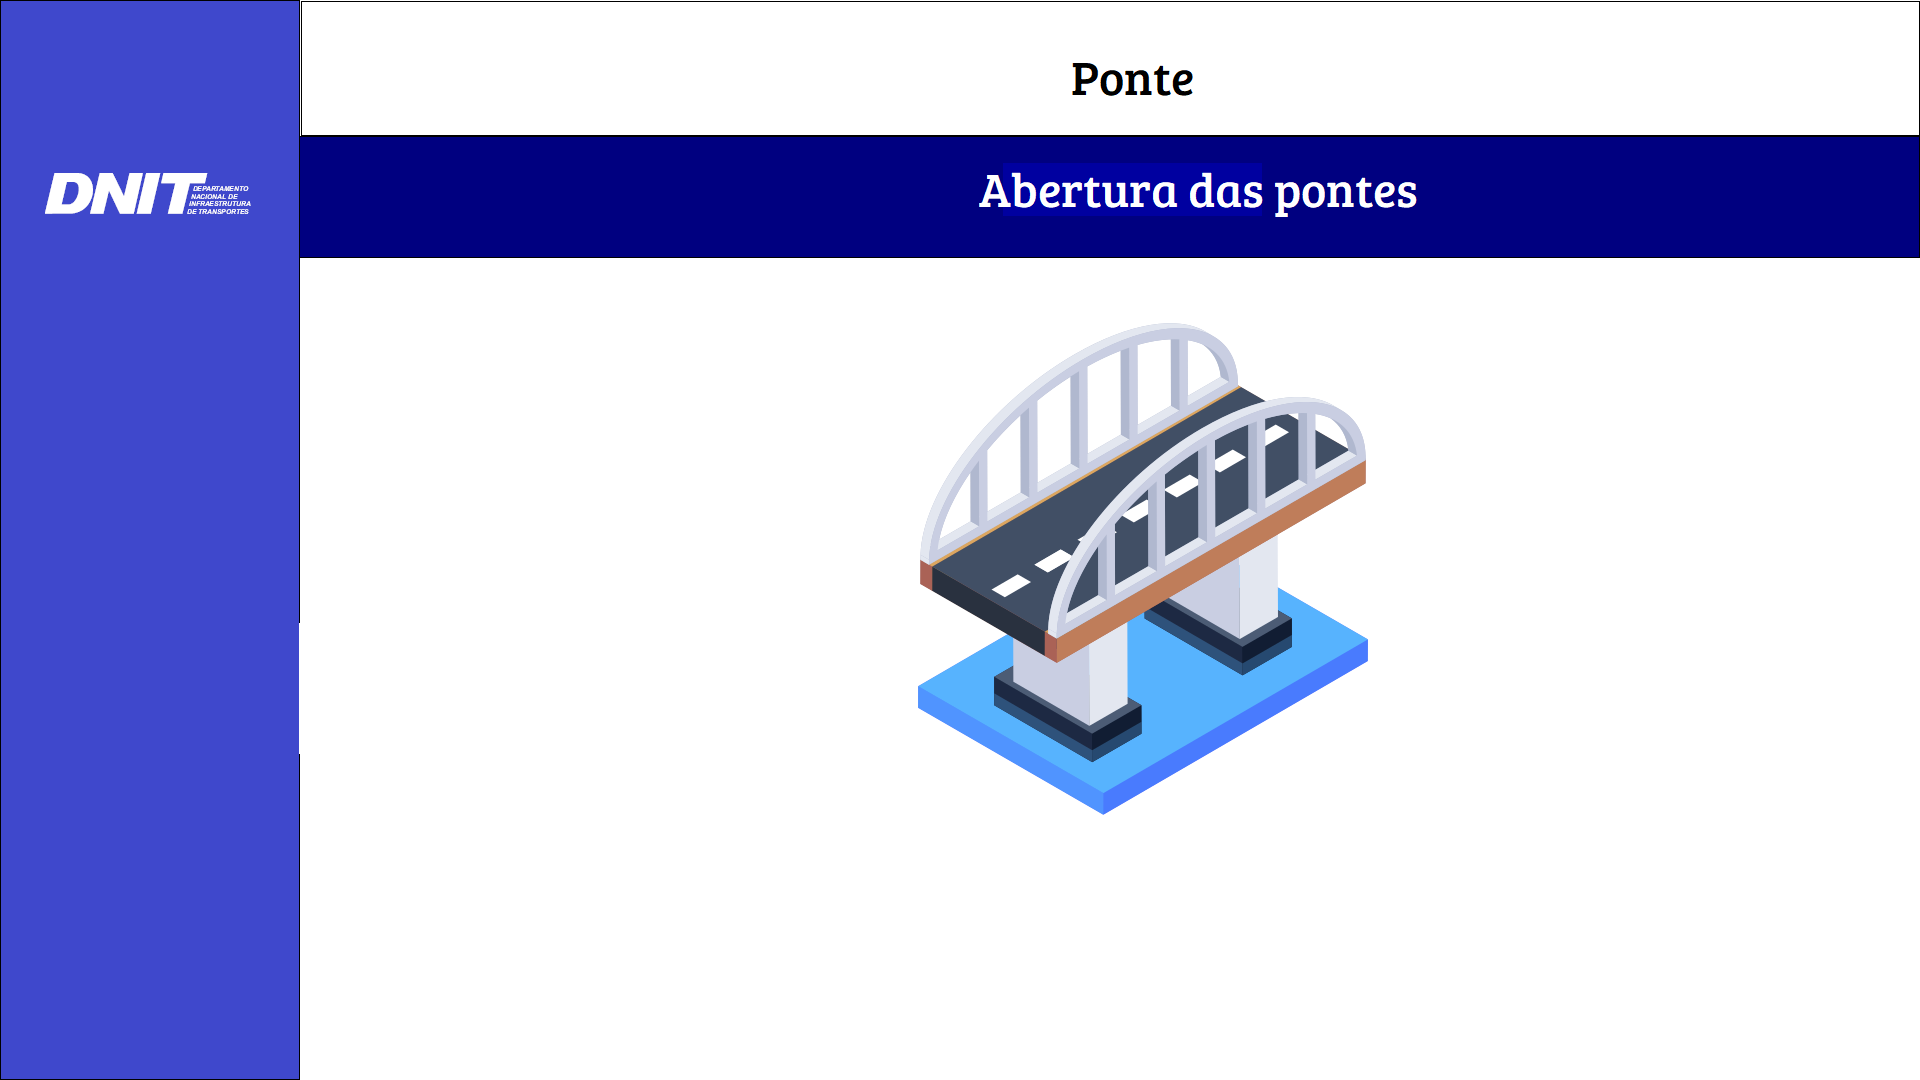
\includegraphics[keepaspectratio=true,scale=0.2]{figuras/Ponte_fim.png}
	\caption{Dashboard da ponte}
\end{figure}


As figuras 22 a 23 mostram o modelo de cada \textit{dashboard} feito para o sistema. O seu interfaceamento se dá pelos ícones criados pelos \textit{dashboards} do sistema. 

\section{Resultados obtidos}

Após configurados os parâmetros no SCADABR, temos que os resultados no geral foram satisfatórios. O controle dos motores dos poços, os semáforos e o motor da ponte foram feitos via \textit{Modbus} com sucesso.

\begin{figure}[h]
	\centering
	\label{fig:circuito_protoboard}
		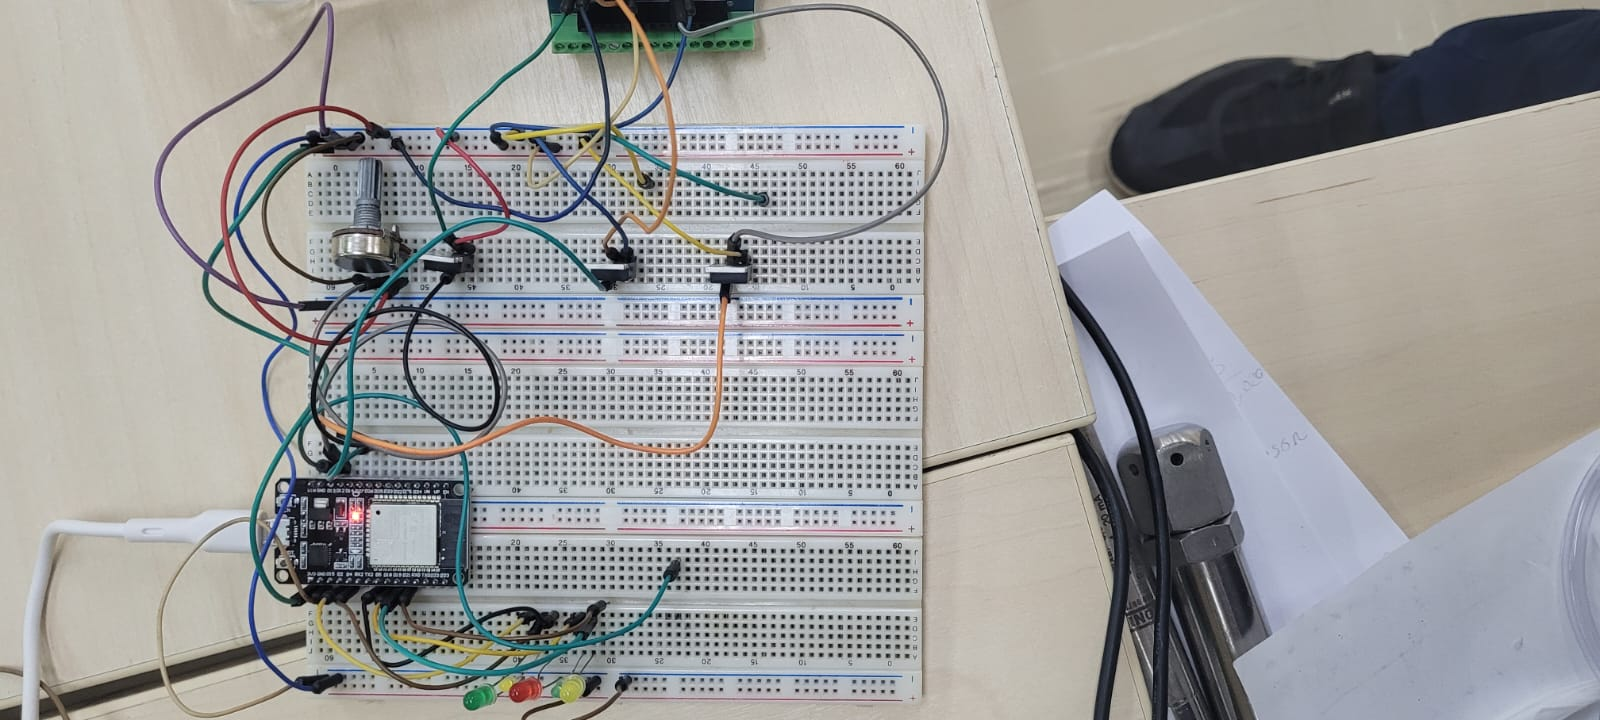
\includegraphics[keepaspectratio=true,scale=0.2]{figuras/circuito.jpeg}
	\caption{Protoboard básica de montagem}
\end{figure}

A figura \ref{fig:circuito_protoboard} mostra o circuito montado na \textit{protoboard}. No caso dos três motores DC, o controle do acionamento foi realizado com comandos \textit{Modbus} enviados ao ESP32, e controlados via supervisório, que por sua vez acionou os motores de forma individual, de acordo com os parâmetros recebidos. Cada motor pode ser iniciado, parado de acordo com os botões acionados via SCADABR

O conjunto de semáforos, composto pelos LEDs, também foi controlado via Modbus. Os sinais de entrada determinaram o estado de cada luz, possibilitando a sincronização das transições entre elas, simulando um ciclo de semáforo típico para gerenciar o tráfego na jusante e montante.

Por fim, o servo motor foi utilizado para controlar o movimento de abrir e fechar a ponte, acionado conforme os comandos recebidos pelo ESP32. Esses comandos definiram o ângulo de rotação do servo, permitindo a execução precisa de movimentos predeterminados.


\begin{figure}[h]
	\centering
	\label{fig:vasilhas}
		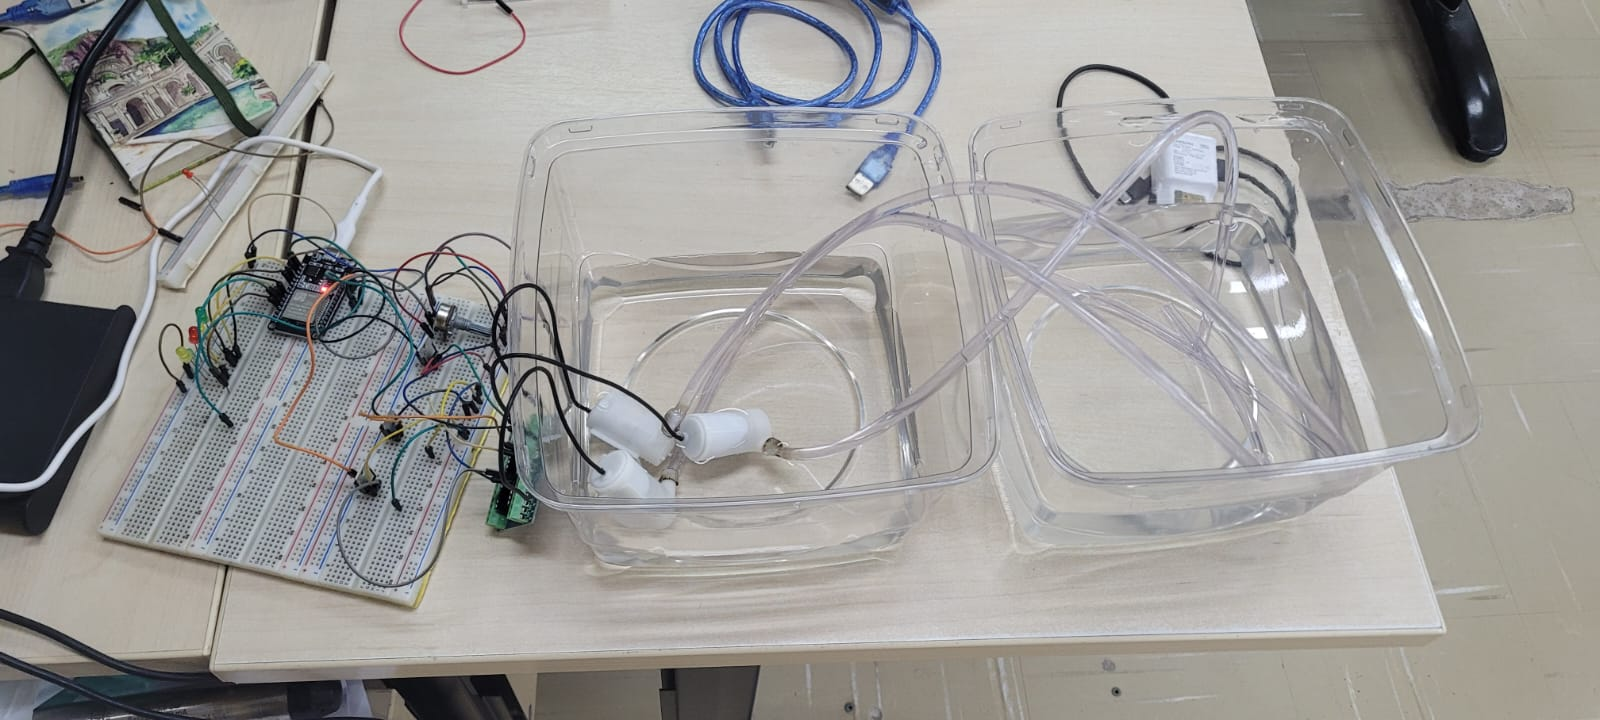
\includegraphics[keepaspectratio=true,scale=0.2]{figuras/vaso_pocos.jpeg}
	\caption{protoboard com as vasilhas simulando os poços}
\end{figure}

Problemas ocorreram , como o motor DC não parar após o comando Modbus. Para isso, foi identificado durante a montagem que a alimentação de 5v da ESP32 estava causando interferência com o acionamento da porta. Para a resolução desse problema foi necessário o uso de uma fonte externa para alimentar os motores de forma segragada ao controlador, sempre interligando os terras existentes. 

Todos esses dispositivos funcionaram de forma coordenada, com o ESP32 gerenciando o envio e recebimento de dados via Modbus e drivers correspondentes controlando a alimentação e movimento dos motores. O sistema permitiu uma operação eficiente e integrada dos dispositivos, com feedback dos estados sendo monitorado continuamente para garantir a precisão do controle e a segurança da operação.


\section{Itens para implementação do projeto}

Para a implementação do projeto nas eclusas, alguns itens são necessários para que ocorra o sucesso na implementação.

\subsection{Instrumentação dos sensores analógicos para eclusa}

Para ler o sensor de nível que mede valores de 4 a 20 mA usando a ESP2, é necessário um circuito de interface para converter essa corrente em uma tensão que possa ser lida pelo controlador, já que os pinos analógicos da esp32 leem tipicamente tensão (0-3,3V).
O circuito para a leitura de interface consiste em um resistor de carga. Para converter a corrente de 4-20 mA em uma tensão que a esp32 possa ler, será usada a transformação tensão/corrente ($R=V/i$). logo, é selecionado um resistor adequado para obter uma tensão entre 0-3,3V quando a corrente varia de 4 a 20 mA.

Com a resolução da transformação, o valor do resistor é de $1,65k \Omega$, a corrente de 4-20 mA se traduzirá em uma tensão na faixa de 1-3,3V está dentro da capacidade de leitura da esp32.


\subsection{Instrumentação dos motores}

O uso de inversores de frequência em bombas e motores é altamente recomendado por diversas razões que beneficiam tanto o desempenho quanto a eficiência dos sistemas. Primeiramente, o inversor de frequência permite um controle mais preciso da velocidade de rotação do motor, ajustando-a de acordo com a demanda real do processo. Isso resulta em uma redução significativa do consumo de energia, uma vez que o motor não precisa operar sempre em sua capacidade máxima. Além disso, o uso do inversor diminui o desgaste mecânico de componentes, como rolamentos e acoplamentos, ao eliminar a necessidade de partidas diretas bruscas, que causam picos de corrente e sobrecarga momentânea. Em bombas, esse controle também evita fenômenos como golpes de aríete, que podem danificar a tubulação. Outro ponto relevante é a flexibilidade operacional, pois os inversores permitem a adaptação a diferentes condições de operação, o que torna o sistema mais versátil e econômico. Portanto, o uso de inversores de frequência é uma solução inteligente para melhorar a eficiência, reduzir custos operacionais e aumentar a vida útil de motores e bombas.

\subsection{Acionamento dos Semáforos}

Para acionar cada uma dessas luzes de forma automática e segura, utilizamos relés de estado sólido, que são dispositivos eletrônicos projetados para ligar e desligar cargas elétricas sem partes móveis, oferecendo maior durabilidade e confiabilidade em comparação aos relés mecânicos.

No sistema de controle do semáforo, a ESP32 irá mandar os sinais através das saídas G5 e G16 a G21, recebe as instruções de tempo e sequência para o acionamento das luzes. Cada relé de estado sólido é conectado a uma das lâmpadas do semáforo, e a função do relé é interromper ou permitir a passagem da corrente elétrica, acionando ou desligando a lâmpada correspondente. O microcontrolador envia sinais elétricos de baixa tensão para o lado de controle do relé, que então permite ou bloqueia a passagem de corrente no circuito de alta tensão, alimentando as lâmpadas do semáforo.

Como os relés de estado sólido são mais rápidos e silenciosos, o acionamento das luzes ocorre de forma suave, sem ruídos de comutação, e sem o desgaste causado por arcos elétricos, comum em relés mecânicos. Além disso, eles apresentam menor aquecimento e oferecem maior eficiência energética. 